\paragraph{Radon transforms}
Define
\[R(f)(t,γ)=∫_{P_{t,γ}}f\]
where $f:ℝ^d→ℝ,\ t∈ℝ,\ γ∈\se^{d-1}⊂ℝ^d$,
\[P_{t,γ}=\{x∈ℝ^d:xγ=t\},\]
i.e.\ the hyperplane orthogonal to $γ$ with distance $tγ$ to the origin. We equip it with the natural $d-1$-dimensional Lebesgue measure, denoted by $m_{d-1}$, which coincides with the $(d-1)$-dimensional Hausdorff measure)
\begin{rem}
	\begin{enumerate}
		\item $f∈C^0_0(ℝ^d)⇒f$ integrable on every $P_{t,γ}⇒R(f)(t,γ)$ defined for every $t,γ$, and $R(f)$ is continuous and compactly supported in $t$.
		\item $f∈L^1(ℝ^d)⇒f$ may fail to be measurable/integrable on some $P_{t,γ}$, which means that $R(f)(t,γ)$ is not defined.
		\item If $f=χ_E$ for $E$ measurable then $R(f)(t,γ)=m_{d-1}(E_{t,γ})$ where $E_{t,γ}=E∩P_{t,γ}$ if $E_{t,γ}$ is measurable.
	\end{enumerate}
\end{rem}
Look instead at the maximal Radon transform: (when should we do this?)
\[R^*(f)(γ)=\sup_{t∈ℝ}|R(f)(t,γ)|\]
We want to study $L^p$-mapping properties of $R$ in order to study regularity of subsets of $ℝ^d$.
\begin{theo} Let $f∈C^0_0(ℝ^d),\ n\geq 3$. Then
	\begin{equation}
		∫_{\se^{d-1}}R^*(f)(γ)\mdσ_γ\leq c(\|f\|_{L^1(ℝ^d)}+\|f\|_{L^2(ℝ^d)})
		\label{eq:mradonbound}
	\end{equation}
\end{theo}
\begin{rem}
	necessary conditions:
	\begin{itemize}
		\item $f∈L^1$: $f(x)=(1+|x|^{d-1})^{-1}∈(L^2\sm L^1)(ℝ^d)$ if $d\geq 3$. $f$ is not integrable in any plane $P_{t,γ}$. ($f∈L^1$ gives global control.)
		\item $f∈L^2$: $f_ε(x)=(|x|+ε)^{-d+δ}$ if $|x|\leq 1,\ δ∈(0,1)$ fixed. Let $ε→0^+$ to see, that \eqref{eq:mradonbound} fails if $\|\cdot\|_{L^2}$ was not on the RHS. ($f∈L^2$ gives local control.)
	\end{itemize}
\end{rem}
Key: interplay between Radon and Fourier transform. $t↦λ∈ℝ$ dual variable. Fourier transform:
\[\wh R(f)(λ,γ)=∫_{-∞}^∞R(f)(t,γ)e^{-2πiλt}\md t\]
\begin{lem} If $f∈C^0_0(ℝ^d),\ γ∈\se^{d-1}$ then 
	\[\wh R(f)(λ,γ)=\wh f(λγ).\]
\end{lem}
\begin{proof}
	\[\wh f(λγ)=∫_{ℝ^d}f(x)e^{-2Yπix(λγ)}\md x=∫_{-∞}^∞(∫_{ℝ^{d-1}}f(u,t)\md u)e^{-2πiλt}\md t=∫_{-∞}^∞(∫_{P_{t,γ}}f)e^{-2πiλt}\md t\]
	where we did the change in coordinates $x=(u,t),\ t=xγ=x_d∈ℝ,\ u=(x_1,…,x_{d-1})∈ℝ^{d-1}$.
\end{proof}
\begin{lem} Let $f∈C^0_0(ℝ^d)$. Then
	\[∫_{\se^{d-1}}(∫_{-∞}^∞|\wh R(f)(λ,γ)|^2|λ|^{d-1}\md λ)\mdσ_γ=2∫_{ℝ^d}|f(x)|^2\md x.\]
\end{lem}
\includepdf[pages=3-6]{V5B7.pdf}
